\documentclass[../main.tex]{subfiles}
\begin{document}
\label{sec:method}

\subsection{The \textit{Galaxy Builder} Zooniverse project}

\textit{Galaxy Builder} is a citizen-science project built on the Zooniverse web platform. It asks volunteers to perform detailed photometric modelling of spiral galaxies (potentially including bulge, disc, bar and spiral arm components). A project of this kind, allowing volunteers to interact with and model data, had never been attempted inside the current Zooniverse web platform before, so this project involved designing and implementing a model rendering\footnote{We use the term rendering in a similar manner to that used for computer graphics: to calculate an image from a model or set of rules.} suite inside the existing Zooniverse front-end code-base. As with all citizen science solutions, we had to not only consider the accuracy of the resulting model, but also user experience and engagement in our design decisions.

The closest relative to this project within the Zooniverse ecosystem was the Galaxy Zoo: Mergers project \citep{Holincheck2016:1604.00435v1}. This project asked volunteers to help match the morphological properties of an image of merging galaxies to a plethora of restricted three-body simulations, in an attempt to identify the initial conditions that could result in the observed morphology. For part of the project, volunteers downloaded a Java applet, which would run restricted three-body simulations and generate output images. Volunteers could mainpulate the model parameters used in the simulation, and vote on simulations which matched a given galaxy merger image or shared important tidal features. A new batch of simulations could then be run and an optimal solution converged on.

In many ways, this iterative workflow was very similar to that used in \textit{Galaxy Builder}: volunteers were asked to manipulate the parameters of a complex astrophysical model in order to identify the most likely solution, in a problem space that traditional computational modelling struggles to solve. However, \textit{Galaxy Builder} operates purely inside a web page and does not make use of additional citizen science projects for model selection (such as the Galaxy Zoo: Mergers' \textit{merger wars} sub-project), instead using unsupervised clustering and computational optimization to identify final models.


\subsubsection{Project Timeline and Development}

The \textit{Galaxy Builder} project was built inside the Zooniverse's \citep{Simpson:2014:ZOW:2567948.2579215} \textsc{Panoptes-Front-End}\footnote{\url{http://github.com/zooniverse/Panoptes-Front-End}} codebase, using Facebook's \textsc{React.js}\footnote{\url{https://reactjs.org/}} framework, as well as WebGL\footnote{\url{https://www.khronos.org/webgl/}} to enable low-latency photometric galaxy model rendering. \textit{Galaxy Builder} entered a Zooniverse beta in late November 2017 and after some user experience improvements and significant code reworking to meet internal standards, the project was launched as an official Zooniverse project on the 24th of April 2018.

A major challenge during development of the project was finding the right balance between keeping the interface and instructions simple enough for volunteers to understand intuitively, while also allowing the freedom and versatility to properly model galaxies. It was also a significant challenge to develop a compelling and simple tutorial for what is one of the most complex projects attempted on the Zooniverse platform. Feedback from expert users was essential to this process as part of the the typical beta trial process for Zooniverse projects\footnote{\url{https://help.zooniverse.org/best-practices/}}.


\subsubsection{The project interface}

The \textit{Galaxy Builder} project prompts volunteers to work through the step-by-step creation of a photometric model of a galaxy (described in detail in Section \ref{section:galaxy-model}). The interface presents a volunteer with three views, which they can switch between at any time: a $r$-band cutout image of a spiral galaxy (see Section \ref{sec:data}), the galaxy model they have created so far, and the residual between their model and image (shown in blue and yellow). A screenshot of the interface can be seen in Figure \ref{fig:interfaceInProgress}, where a residual image is shown.

\begin{figure*}
  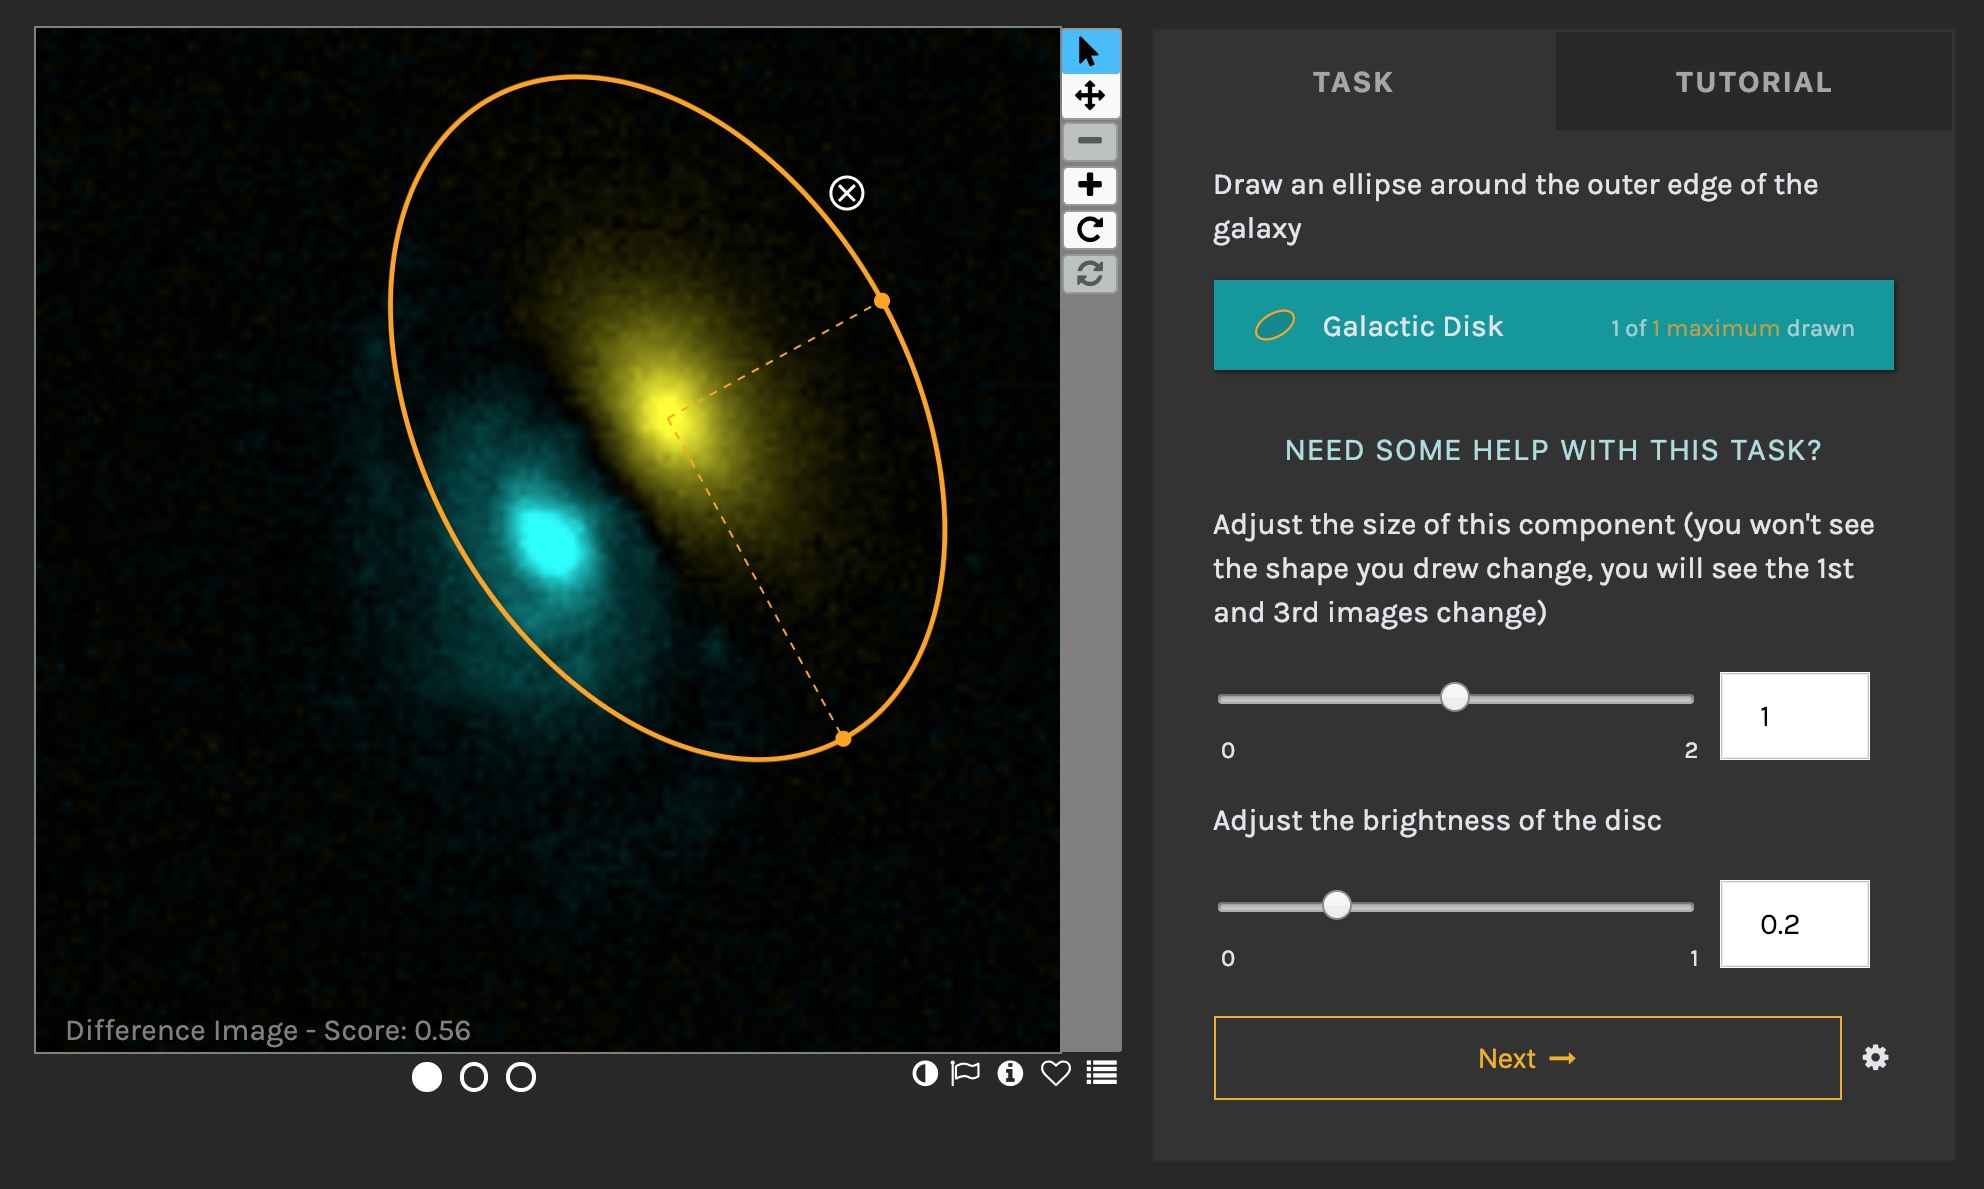
\includegraphics[width=17.7cm]{images/interfaceInProgress.jpg}
  \caption{The \textit{Galaxy Builder} interface. The residual image is being shown, and the volunteer is on the ``Disc'' task. The drawn disc component (yellow) is offset from the galaxy image (blue) to demonstrate the positive and negative residuals. Where the image equals the model the residual is black. The dots below the residual image allow the user to switch images. The icons to the right allow panning and zooming of the image (rotation was not functional for this project). The icons to the bottom right of the image allow colour inversion of the galaxy cutout, flagging of the image as inappropriate, inspection of galaxy metadata (i.e. sky position, link to SDSS SkyServer), ability to save the image as a favourite and to add to a Zooniverse ``collection''. The Score shown in the bottom left of the image is calculated using Equation \ref{eqn:gal_score} and is a rough goodness-of-fit measure.}
  \label{fig:interfaceInProgress}
\end{figure*}


The workflow is designed so that volunteers slowly subtract increasing amounts of light from the galaxy, as can be seen in Figure \ref{fig:residualsStepByStep}. A tutorial is available which contains a step-by-step guide to completing a classification. At each step volunteers are asked to first draw a simple isophote, and then make use of a series of sliders to adjust the parameters of the model component (see Section \label{section:galaxy-model} for more information).

Volunteers are also guided by a ``score'', which is tied to the residuals and chosen to increase from zero to some arbitrary value depending on the galaxy; a less noisy and more easily modelled galaxy will have a higher maximum score. To map a residual image to a final score shown to volunteers we used

\begin{equation}
  \label{eqn:gal_score}
    S = 100 \exp\left(\frac{-A}{N}\sum_{i=0}^N\frac{\text{arcsinh}^2\left(\,|\text{y}_i - M_i|\ /\ 0.6\right)}{\text{arcsinh}\,0.6 }\right),
\end{equation}

where $N$ is the total number of pixels, $y$ is the cutout of the galaxy, normalized to a maximum value of 1 ($y = \text{cutout}/\text{max}(\text{cutout})$), $M$ is the model calculated by volunteers and $A=300$ is an arbitrary choice of scaling chosen based on a handful of test galaxies.

This score has the advantage of being easy (and fast) to generate from the residual image shown to voluteers (which was Arcsinh-scaled in a manner described by \citealt{Lupton2003:astro-ph/0312483v1}), however it is quite sensitive to small deviations of the model from the galaxy.

\begin{figure}
  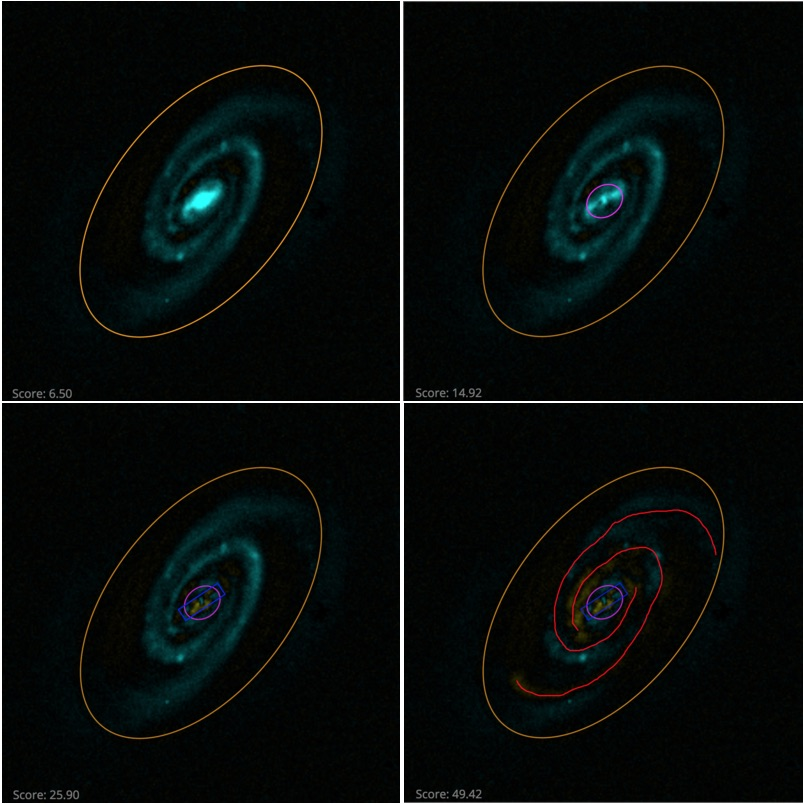
\includegraphics[width=8cm]{images/residualProgress.jpg}
  \caption{Figure demonstrating the desired result of each step of the modelling process, as seen from the residual image provided to volunteers. The top left panel shows the galaxy after only a disc component has been added: the top right contains a disc and a bulge; the bottom left has a disc, bulge and bar; the bottom right is the finished model with a disc, bulge, bar and spiral arms. The images shown is SDSS J104238.12+235706.8. This brightness and contrast of this image have been edited to improve visibility in print.}
  \label{fig:residualsStepByStep}
\end{figure}


\subsection{Sample Selection: Images and Ancillary Data}
\label{sec:data}

\textit{Galaxy Builder} finds a niche with complex, multi-component galaxies. As such, the sample should be selected to have these features. The original sample proposed for the \textit{Galaxy Builder} project aimed to mirror the \textit{stellar mass-complete sample} in \citet{2017MNRAS.472.2263H}. This was a sample of face-on spiral galaxies, with and without bars, complete in  stellar mass.

The morphological information required to select spiral galaxies came from the public data release of Galaxy Zoo 2 (\citealt{Willett2013:1308.3496v2}, hereafter GZ2). Each response to a GZ2 morphology question is allocated a $p$ value ranging from 0 to 1, where 0 indicates no volunteers responed positively to that question and 1 indicates all volunteers who classified that galaxy responded positively (i.e. $p_\text{bar} = 0.5$ would indicate $50\%$ of volunteers said a bar was present in a galaxy). Photometric measurements used for selection came from the NASA-Sloan Atlas (\citealt{2011AJ....142...31B}, hereafter NSA). The \textit{stellar mass complete sample} is constructed using the set of criteria detailed in Table \ref{table:sample_selection}.

\begin{table*}
  \centering
  \caption{The selection criteria used in \citet{2017MNRAS.472.2263H} to create the \textit{stellar mass-complete sample} of 6222 spiral galaxies.}
  \begin{tabular}{ |l|c| }
    \hline
    Description & Value\\
    \hline
    Face-on spiral morphological selection. & GZ2 $p_\text{features} \cdot p_\text{not edge on} \cdot p_\text{spiral} \ge 0.5$ \\
    Redshift limits. & $0.02 < z < 0.055$ \\
    Face-on galaxy selection using g-band axial ratio. & $(b/a)_g > 0.4$ \\
    Volume correction. & $9.45 < \log(M_* / M_\odot) \le 11.05$ \\
    Computation of stellar mass completeness limits using & $2.07\log(z) + 12.64 < \log({M_* / M_\odot}) < 2.45\log(z) + 14.05$ \\
    the method of \citet{Pozzetti2009:0907.5416v2} and limits calculated & \\
    by \citet{2017MNRAS.472.2263H}. & \\
    \hline
  \end{tabular}
  \label{table:sample_selection}
\end{table*}

The \textit{stellar mass-complete sample} was split into smaller sub-samples, each containing 100 galaxies. In an iterative process, each sub-sample was chosen to contain 60 of the lowest redshift galaxies and 40 random galaxies of those remaining in the sample. This was done to account for the unknown rate at which volunteers would provide classifications. In the first two sets of 100 galaxies, 1\% of galaxies (i.e. 2 images) failed to run through the image preparation process, due to an error when attempting to montage multiple frames. The root cause of this error is unknown, but it leaves a sample of 198 galaxies with images that are considered in this paper.

\subsubsection{Image and modelling metadata extraction}

The galaxy data shown to volunteers in the \textit{Galaxy Builder} project came in two forms: A gray-scale image cutout of the galaxy and a JSON file containing rendering information for the web-interface.

Both forms of data were obtained using a similar process:

\begin{itemize}
\item A montage of multiple r-band corrected frames from the SDSS DR13 \citep{2017ApJS..233...25A} data release was created. To combine multiple FITS images, we made use of Astropy \citep{2018AJ....156..123T}, and the \textsc{Montage} \citep{2010arXiv1005.4454J} software package.
\item This montage was cropped to four times the Petrosian radius of the galaxy.
\item The \textsc{SExtractor} software \citep{source-extractor} was used to identify regions containing secondary sources (foreground stats, other galaxies) and generate a mask.
\item A PSF was obtained from the relevant Sloan r-band \texttt{psField} file, extracted at the central position of the galaxy \citep{2002AJ....123..485S}.
\item The JSON file was written containing the cut-out data and the 2D boolean mask obtained from the source extraction process. This file also contained other metadata needed for the rendering process (PSF, the size of the PSF array, and the width and height of the image).
\item Another JSON file containing simply the information used to render the volunteer's model (image size and PSF) was created.
\item An arcsinh-stretch was applied to the masked cutout (as described by \citealt{Lupton2003:astro-ph/0312483v1}). It was then saved as a grey-scale image.
\end{itemize}

The decision to use r-band images in our subject set was due to its higher signal-to-noise than other bands.

Once a sub-sample had been created, the Zooniverse's \textsc{panoptes-python-client}\footnote{\url{https://github.com/zooniverse/panoptes-python-client}} was used to upload them as a subject-set to the Zooniverse.

A separate stacked image and sigma image was calculated for the r-band corrected frames present in the montage, as described in Appendix \ref{appendix:frame_stacking}. These were not caluclated using \textsc{Montage} as its reprojection step does not conserve errors. These images were not shown to volunteers but were used for model tuning and comparison.


\subsection{Choice of Retirement limit}
\label{sec:retirement-limit}

Initially, 10 classifications were collected per galaxy, however preliminary analysis indicated this number of independent answers was insufficient to create reliable and reproducable aggregate classifications. For this reason, a hand-picked sample of 56 galaxies was then re-activated with a retirement limit of 30 classifications per galaxy. This sample was chosen by eye to be a relatively diverse set of galaxies, most with prominent spiral features including grand-design and flocculent arms. Its purpose was to allow the development of the aggregation methodology.

Once this hand-picked sample was completed, and it had been determined that 30 classifications per galaxy was sufficient, the remaining galaxies from the initial two sub-samples were re-activated, as well as a repeat of the first sub-sample (hereafter the \textit{validation subset}) to measure volunteer consistency. This paper focuses on these 198 galaxies (presented in \textit{Galaxy Builder} as 296 separate images) in order to explain the method used, and test the reliability of the models obtained. The \textit{Galaxy Builder} project is still active on the Zooniverse website as of the time of writing and continues to collect classifications for further samples of galaxies.


\subsection{The Galaxy Model}
\label{section:galaxy-model}

The model chosen was largely based on the components and methodology described in \citet{galfit-paper}. The model components consisted of:
\begin{enumerate}
\item An exponential, elliptical disc.
\item An elliptical S\'ersic bulge, with $n$ chosen by volunteers and allowed to vary from 0.5 to 5.
\item A S\'ersic bar with a ``boxiness'' modifier (as described in \citealt{galfit-paper}).
\item Any number of freehand poly-line spiral arms.
\end{enumerate}

Each spiral arm is modelled using a poly-line drawn by the volunteer. The brightness of a spiral arm at any point is given by the value of a Gaussian centred at the nearest point on any drawn poly-line, with volunteers able to choose the Gaussian width and peak brightness using sliders. Radial falloff was added by multiplying by the value of the previously added exponential disc, though volunteers could change the half-light radius of this falloff disc.

The modelling code ignores masked regions identified as secondary sources by \textsc{SExtractor}. It over-samples the bulge, disc and bar components by a factor of five and performs PSF convolution using a PSF obtained from the relevant Sloan r-band \texttt{psField} file, extracted at the central position of the galaxy \citep{2002AJ....123..485S}.


\subsection{Reprojection of Classifications into original SDSS Frame Coordinates}

In order to properly account for errors and as part of the data reduction process, we transform all classifications recieved for a galaxy from the coordinate space of the \textsc{Montage}-created cutouts back into the WCS of the original frames. This was motivated by the need for accurate sigma images, which it is not possible to create for the cutout created using \textsc{Montage} due to the reprojection having a smoothing effect on the background noise, despite being flux-conserving overall.


\subsection{Classification Aggregation Methodology}

In this Section, we will use the galaxy UGC 4721, a two-armed barred spiral galaxy at $z=0.02086$ classified by \citet{deVaucouleurs1991} as SBcd, to illustrate the data reduction and aggregation methodology. For UGC 4721 we received 32 classifications, containing 28 discs, 24 bulges, 17 bars and 47 drawn spiral arm poly-lines. These annotations can be seen in Figure \ref{fig:drawn_shapes}, overlaid on the greyscale r-band image of the galaxy.

\begin{figure*}
  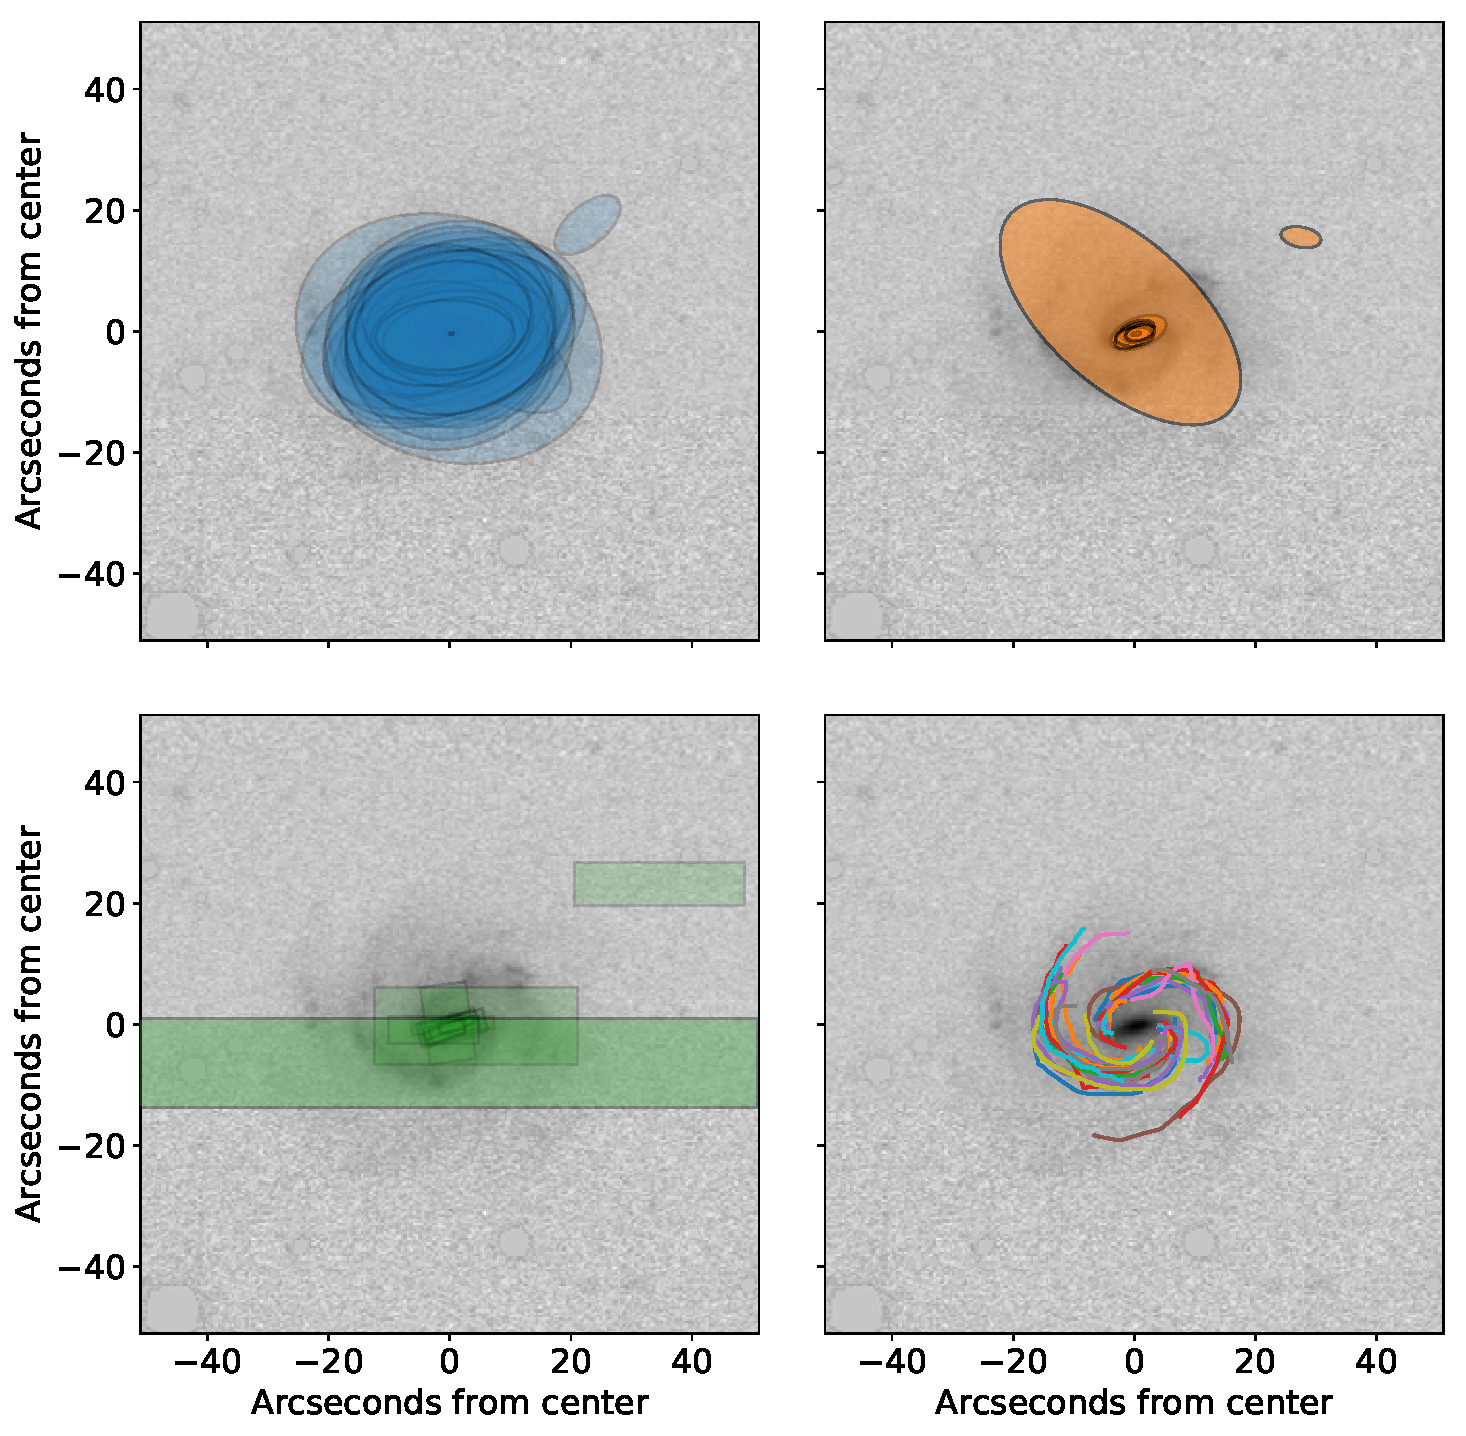
\includegraphics[width=17.3cm]{images__method/drawn_shapes.pdf}
  \caption{Components drawn by volunteers for UGC 4721. The top left panel shows drawn discs, top right shows drawn bulges, bottom left shows drawn bars and bottom right shows drawn spiral arms.}
  \label{fig:drawn_shapes}
\end{figure*}

\subsubsection{Best Individual Classification}

As \textit{Galaxy Builder} is primarily asking volunteers to solve a complicated regression problem, it is possible to identify the classification provided for each galaxy with the best residual, and assume that this classification has roughly found the globally optimal model. We make use of the model's $\chi_\nu^2$ (Equation \ref{eqn:chisq}, as used by \textsc{Galfit}) in units of nanomaggies, to score the volunteer models\footnote{Note that this is not the score shown to volunteers, Equation \ref{eqn:gal_score}.}.

\begin{equation}
  \label{eqn:chisq}
  $$\chi_\nu^2 =\frac{1}{N_\mathrm{dof}}\sum_{x=1}^{nx}\sum_{y=1}^{ny}\frac{\left(f_\mathrm{data}(x, y) - f_\mathrm{model}(x, y)\right)^2}{\sigma(x, y)^2}$$
\end{equation}

We note that it is impossible to calculate the degrees of freedom of a nonlinear model such as a S\'ersic profile, and as such $\chi_\nu^2$ is not an appropriate measure for model comparison \citep{2010arXiv1012.3754A}. We aproximate $N_\mathrm{dof} \sim nx \times ny$ as the number of pixels present in an image, as the number of model paramters is insignificant in comparison. Values of $\sigma$ were taken from the sigma image for the galaxy.


\subsubsection{Aggregation of Volunteer Models}
\label{sec:aggregation_of_volunteer_models}

As we have multiple independent answers for each parameter and component, we can also combine these to find an aggregated answer. Aggregate model calculation was done on a component-by-component basis, rather than per classification, i.e. clustering of discs was performed independently to that of bulges, bars and spirals. Clustering was performed using the Jaccard distance measure (also known as the intersect-over-union distance, or IOU distance), which is a simple metric determining the relative shared area of two shapes:

\begin{equation}
d_J(A, B) = 1 - \frac{|A \cap B|}{|A \cup B|}.
\end{equation}

The algorithm chosen to perform clustering was the density-based spatial clustering of applications with noise (DBSCAN, \citealt{dbscan}) algorithm, due to its robustness and speed. We made use of Scikit-learn \citep{scikit-learn} to implement the algorithm. In DBSCAN the core of a cluster is defined as a group of at least \texttt{min\_points} that are all within a distance \texttt{eps} of each other. Additionally, any points within a distance \texttt{eps} of a cluster's core are also associated with the cluster.
The values of \texttt{eps} and \texttt{min\_points} for the disk and bulge were chosen by visually inspecting the resulting clustering results. The value of \texttt{eps} used to cluster bars was tuned such that the aggregate model best agreed with GZ2 $p_\mathrm{bar}$ ($p_\mathrm{bar} < 0.2$ implying no bar and $p_\mathrm{bar} > 0.5$ implying a definite bar). The values used can be seen in Table \ref{table:dbscan_params}. Bar with axis ratios greater than 0.6 were removed from the pool as this was deemed unphysical.

\begin{table}
  \centering
  \caption{The clustering parameters used for the disc, bulge and bar components present in \textit{Galaxy Builder}}
  \begin{tabular}{ |c|c|c| }
    \hline
    component & \texttt{eps} & \texttt{min\_points} \\
    \hline
    Disc & 0.3 & 5 \\
    Bulge & 0.3 & 3 \\
    Bar & 0.385 & 3 \\
    \hline
  \end{tabular}
  \label{table:dbscan_params}
\end{table}

For shapes clustered in this way, we define the aggregate component to be the shape which minimises the sum of Jaccard distances to each of the shapes in the cluster. For our example galaxy, UGC 4721, clustered and aggregate components can be seen in Figure \ref{fig:mean_shapes}.

\begin{figure*}
  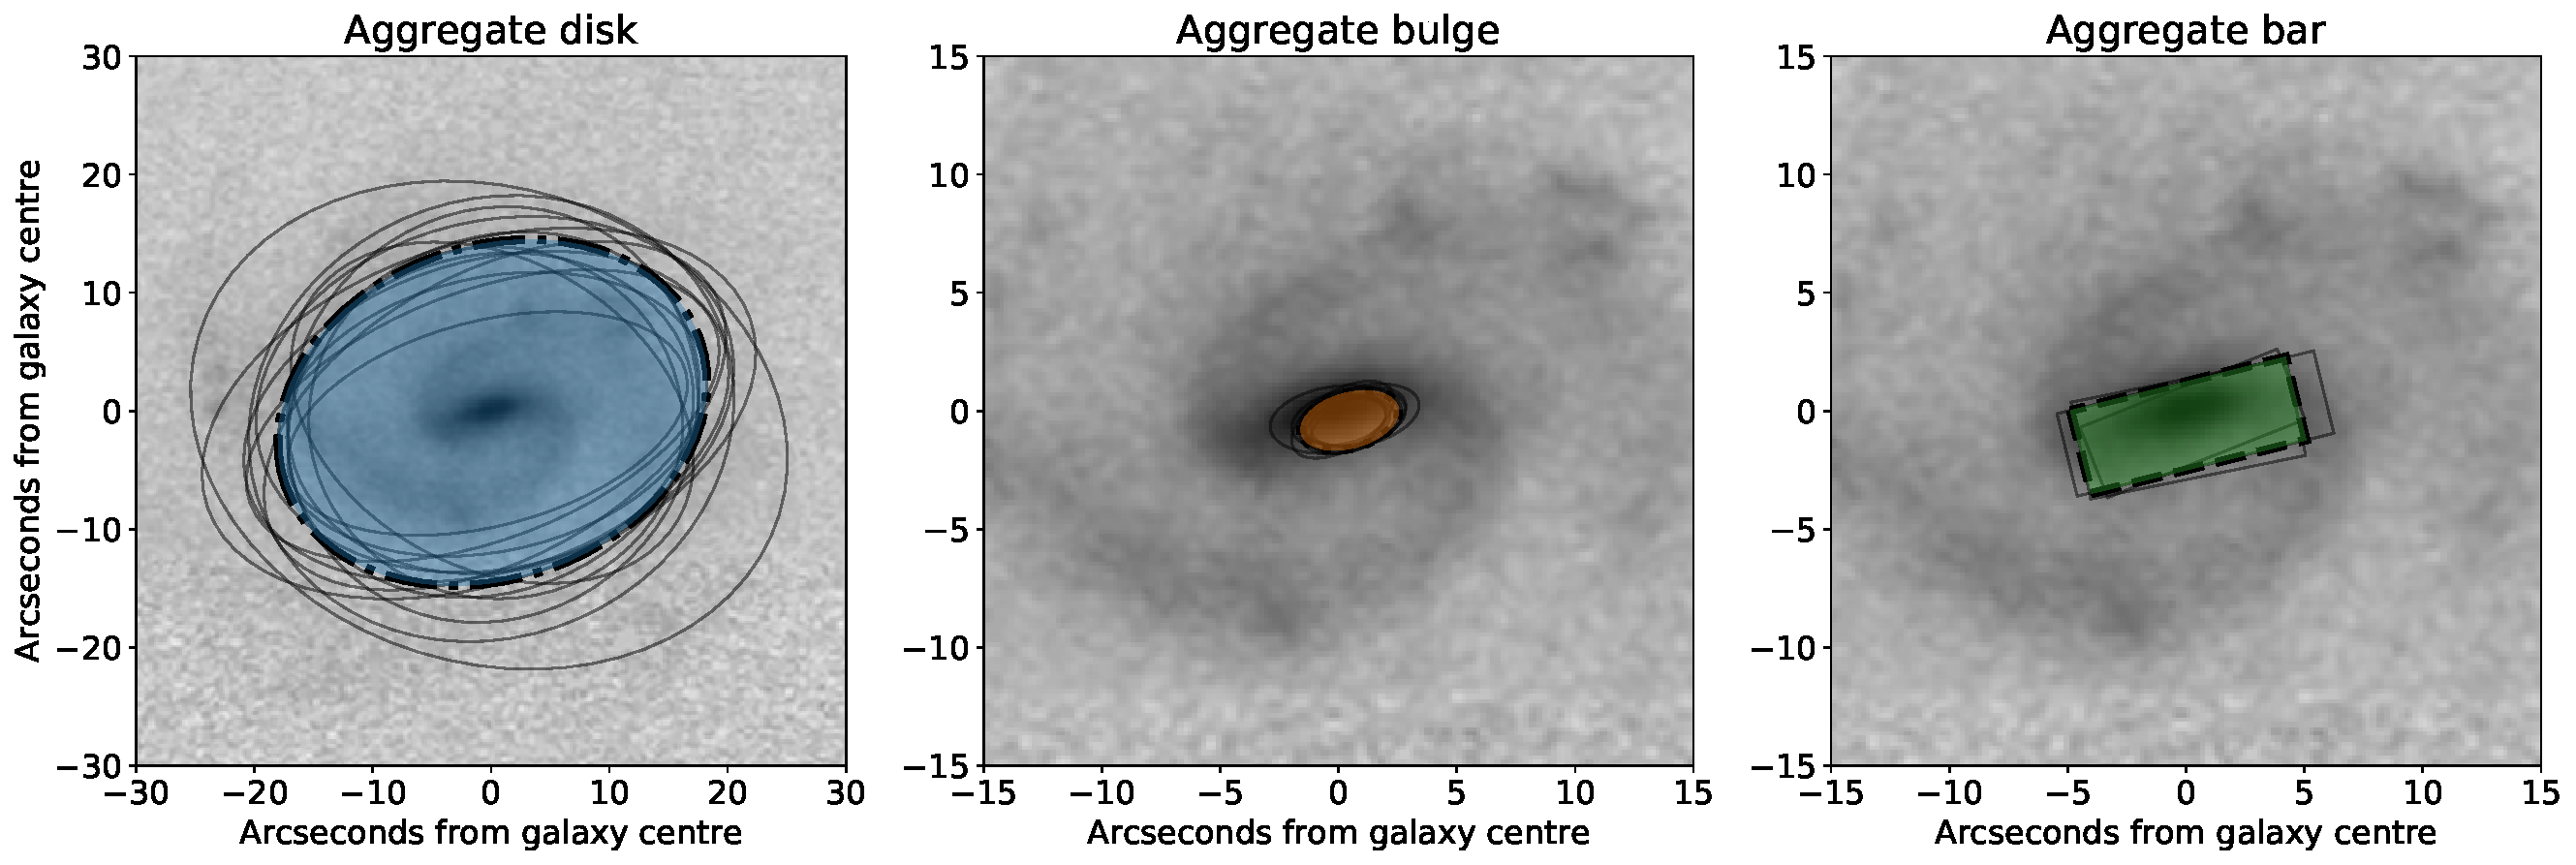
\includegraphics[width=17.3cm]{images__method/mean_shapes.pdf}
  \caption{Calculated aggregate components for UGC 4721. The aggregate disc is shown using a dot-dashed line and blue fill in the first panel, the aggregate bulge with a dotted line and orange fill in the second panel and the aggregate bar using a dashed line and green fill in the third panel.}
  \label{fig:mean_shapes}
\end{figure*}

To cluster drawn spiral arms, we define a custom separation measure to represent how far away one poly-line is from another. This measure was chosen to be the mean of the squared distances from each vertex in a poly-line to the nearest point (vertex or edge) of another poly-line, added to the mean of the squared distances from the second poly-line to the first. A mathematical description of this measure can be found in Appendix \ref{appendix:clustering_maths}. We make use of this separation measure inside the DBSCAN algorithm to cluster these drawn lines, after removing any self-intersecting drawn arms (as this was deemed an easy method to filter out ``bad'' classifications).

Once spiral classifications on a galaxy have been clustered into the physical arms they represent, the points are deprojected using the axial ratio from a 2D, single-component S\'ersic fit in r-band, provided in the NSA catalogue \citep{2011AJ....142...31B}. The deprojection method assumes a thin disc and stretches the elliptical minor axis to match the major axis.

Deprojected points within each drawn poly-line are converted to polar coordinates and unwound using \texttt{numpy.unwrap} to allow model fitting. These unwound points are then cleaned using the Local-outlier-factor algorithm (LOF, \citealt{local-outlier-factor}). For each arm in the cluster, the LOF algorithm was trained on all points not in that arm, and then used to predict whether each point in the arm should be considered an outlier. In this way we clean our data while respecting its grouped nature. The points removed as outliers for the example galaxy are shown in Figure. \ref{fig:LOF_cleaning}.

\begin{figure}
  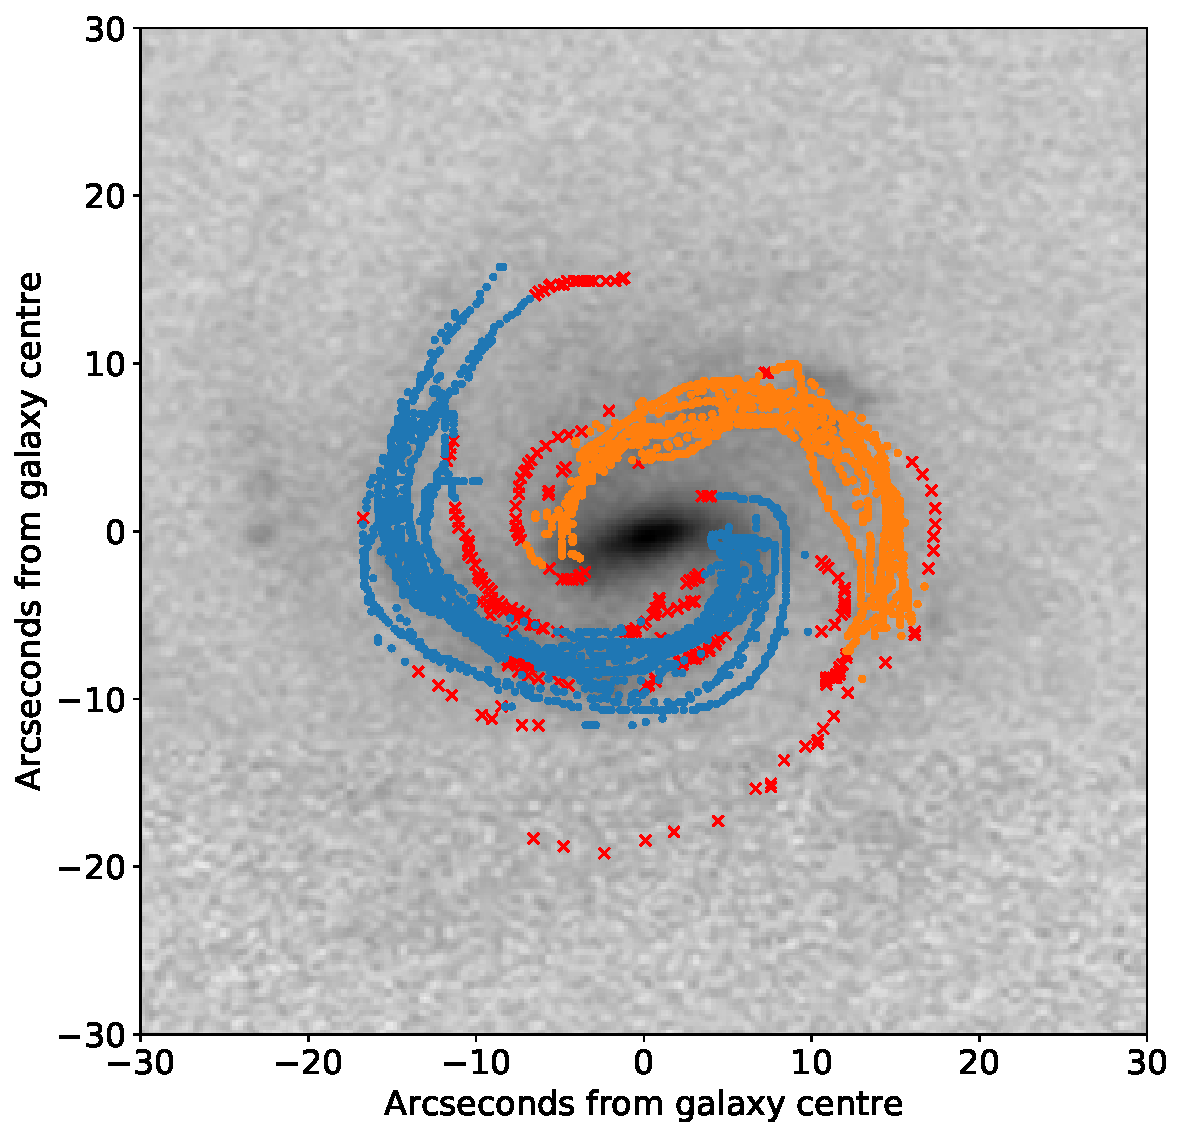
\includegraphics[width=8cm]{images__method/LOF_cleaning.pdf}
  \caption{Point cleaning for the spiral arm clusters for UGC 4721. Points identified as outliers are displayed as red crosses, points used to fit log spirals are orange and blue dots.}
  \label{fig:LOF_cleaning}
\end{figure}

For each arm cluster in each galaxy, a logarithmic spiral model was fitted using Bayesian Ridge Regression, performed using the Scikit-learn python package. Hyperpriors on the noise parameter were chosen by fitting a truncated gamma distribution \citep{2014arXiv1401.0287Z} to the spiral width slider values returned by volunteers (ignoring sliders left at the default or moved to the extremes of allowed values). To obtain a single value for the pitch angle of a galaxy, we take the length-weighted average pitch angle of all arms detected in the galaxy (as used by \citealt{Davis2014:1402.1910v1}).

The final galaxy model for UGC 4721 obtained through aggregation can be seen in Figure \ref{fig:aggregate_model}.

\begin{figure}
  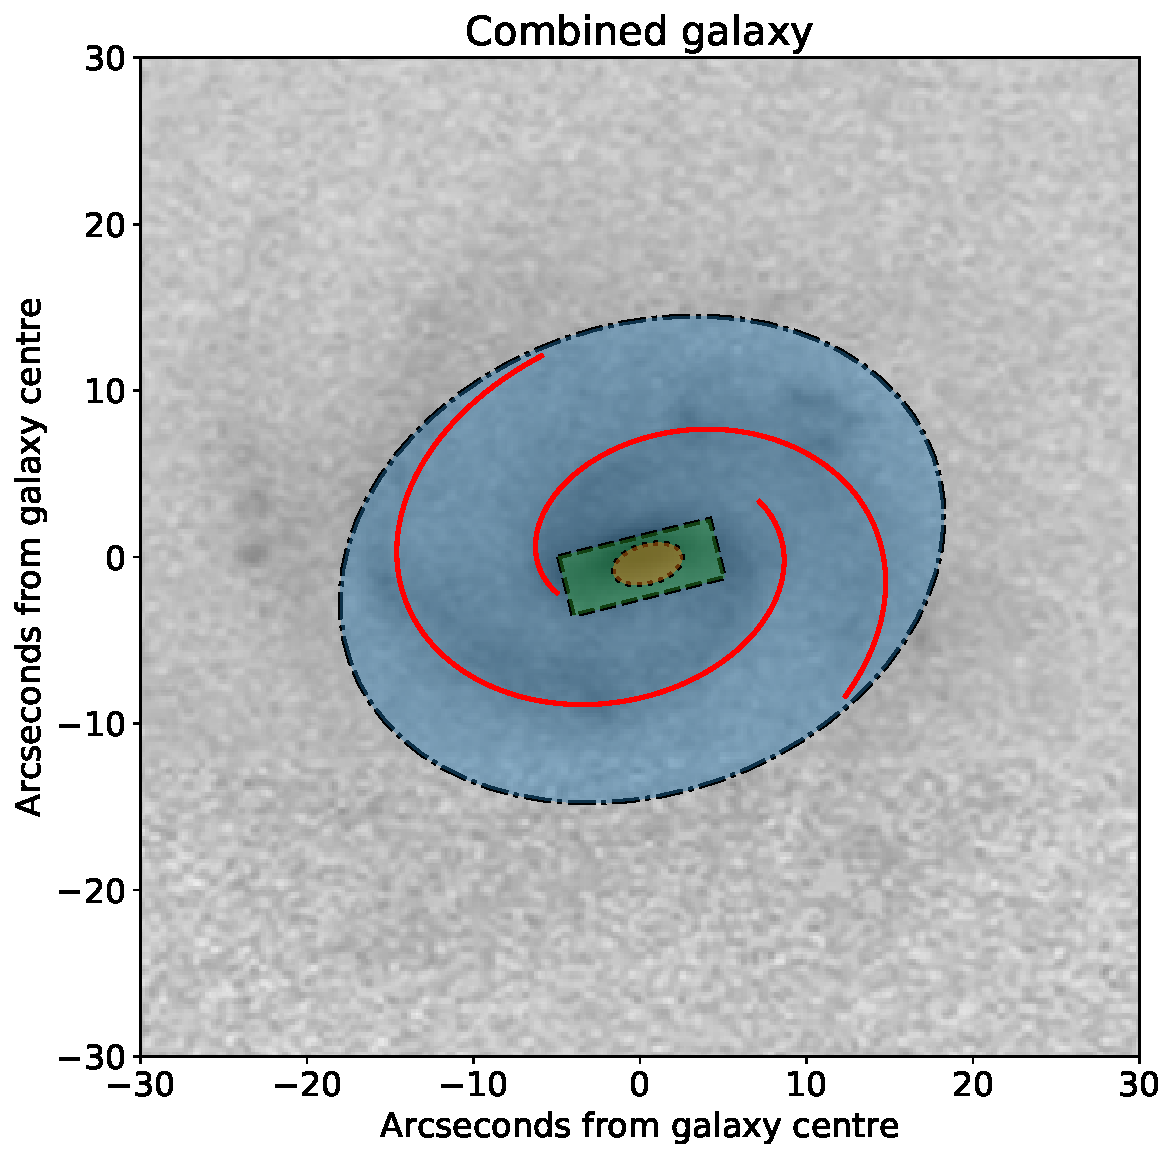
\includegraphics[width=8cm]{images__method/aggregate_model.pdf}
  \caption{Resulting aggregate bulge + disc + bar + spiral arms components for UGC 4721. The disc is shown in blue with a dashed outline, the bulge in orange with a dash-dot outline, the bar in green with a dotted outline, and the spiral arms in red.}
  \label{fig:aggregate_model}
\end{figure}

\subsection{Model Tuning}

As mentioned above, the need for a numerical fit to fine-tune parameters of \textit{Galaxy Builder} models was anticipated. This tuning was performed using the L\_BFGS-b algorithm \citep{doi:10.1137/0916069}, implemented in \textsc{Scipy} \citep{scipy-paper}, to minimize the model's $\chi_\nu^2$ (Equation \ref{eqn:chisq}). Parameter bounds were chosen to be as uninformative as possible, while preventing catastrophic fitting failure where possible. All parameter bounds can be found in Table \ref{table:bad_values}. Tuning was performed on both the best individual models and the aggregate models, and the resulting $\chi_\nu^2$ values were almost identical, suggesting convergence to the same minima. After tuning, some models display the problematic behaviour noted in \citet{2018MNRAS.473.4731K}, including bar ellipticity increasing beyond 0.5 and bulge and bar effective radius increasing to be larger than the disk. We note one case where the best individual model contains a bar being used to mask a point source that was not identified in the masking process.

The tuning process sucessfully lowered model $\chi_\nu^2$ values to between 1 and 5 for both best individual and aggregate models. Models and residuals for the tuned best individual and aggregate models for our example galaxy are shown in Figure \ref{fig:bi_vs_agg_comparison}. We still see spiral structure present in the residuals, as the spiral arms were not positioned perfectly (especially the spiral start and end points). We reccommend that future methods attempt to optimize these values.

\begin{figure}
  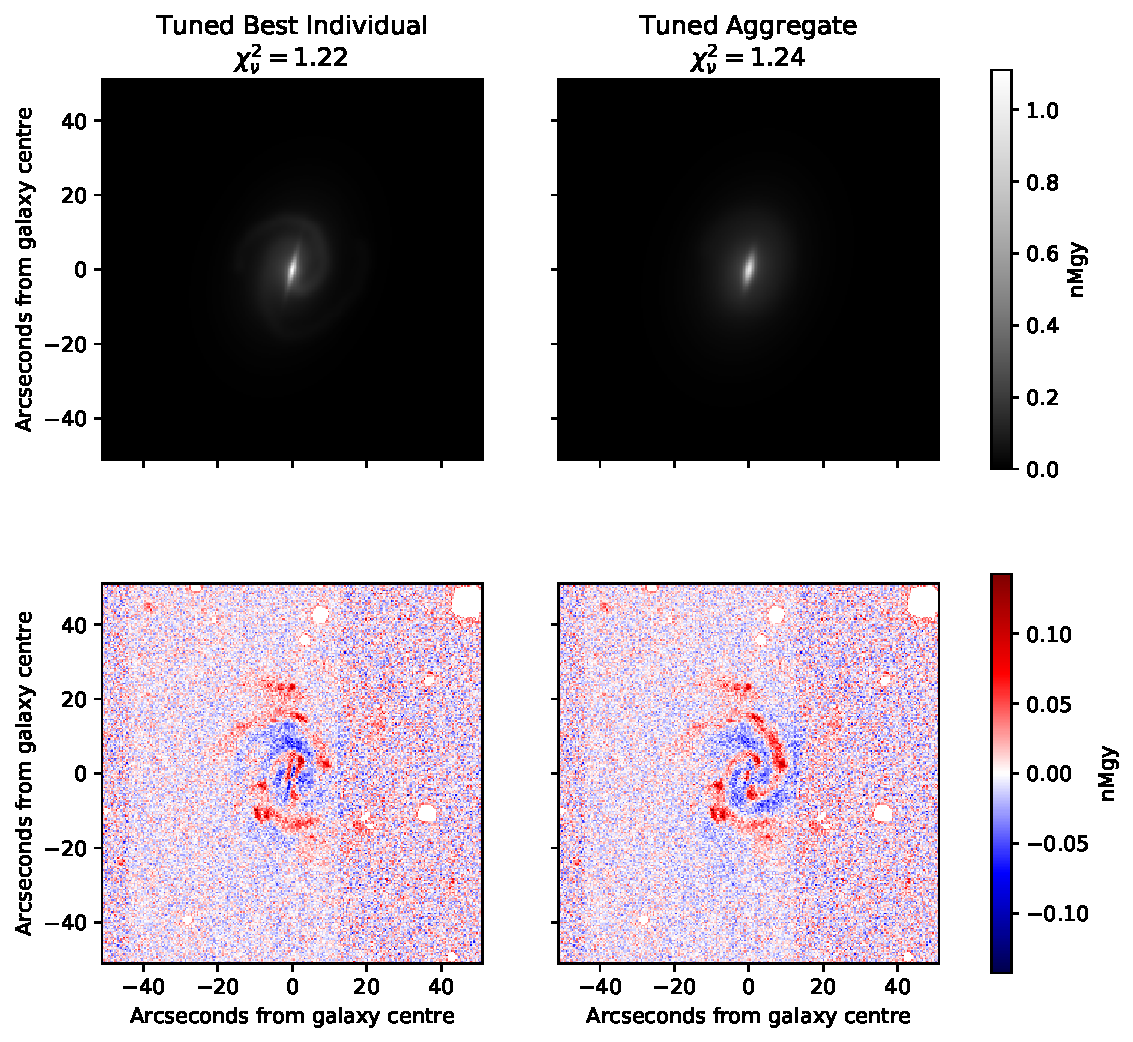
\includegraphics[width=8cm]{images__method/bi_vs_agg_comparison.pdf}
  \caption{Tuned best individual and aggregate models, and their residuals for UGC 4721. The top two panels show the models, with the tuned best individual model on the left and the tuned aggregate model on the right. Bottom panels show the corresponding residuals, where red indicates oversubtraction of the galaxy and blue indicates undersubtraction.}
  \label{fig:bi_vs_agg_comparison}
\end{figure}


\subsection{Error Estimation}
\label{sec:error_estimation}

The uncertainties reported by many software fitting packages (\textsc{Galfit} and \textsc{MegaMorph} from the above list) are lower estimates on the real uncertainty, due to secondary sources not being modelled, flat-fielding errors and incorrect models \citep{2010AJ....139.2097P}. Other packages such as \textsc{Gim2d} and \textsc{Profit} attempt to fully model posterior distributions and so produce more representative uncertainties, however this comes with a larger computational cost and configuration complexity.

As all shapes in a cluster can be viewed as volunteers' attempts at modelling the underlying component, the sample variance of the parameters of these shapes can be used as a good approximation of the underlying variance of the component. Figure \ref{fig:mean_shapes} illustrates the variance in clustered shapes for our example galaxy (UCG 4721). Effective radii generally had relative errors of around 10\% and axis ratios show an absoulute error of around $0.10$. Parameters dictated by sliders show much larger and less consistent errors, potentially due to their impact being conceptually harder for volunteers. It is therefore possible that slider errors should be treated as a measure of volunteer confidence rather than a measure of the posterior. A table detailing all errors on parameters is provided in the appendix (Table \ref{table:error_values}).

\end{document}
